\documentclass[tikz,border=15pt]{standalone}
\usepackage{tikz}
\usetikzlibrary{shapes.geometric, arrows.meta, positioning}

\tikzset{
    register/.style={
        rectangle, draw=black, thick,
        minimum width=1cm, minimum height=0.85cm,
        fill=white, font=\small\ttfamily
    },
    alu/.style={
        rectangle, draw=black, thick,
        minimum width=0.95cm, minimum height=0.75cm,
        fill=white, font=\small
    },
    wire/.style={draw=black, thick, -Stealth},
    buswidth/.style={font=\scriptsize, fill=white, inner sep=2pt},
    logic/.style={
        rectangle, draw=black, thick, rounded corners=3pt,
        minimum width=0.8cm, minimum height=0.75cm,
        fill=gray!10, font=\small
    }
}

\begin{document}
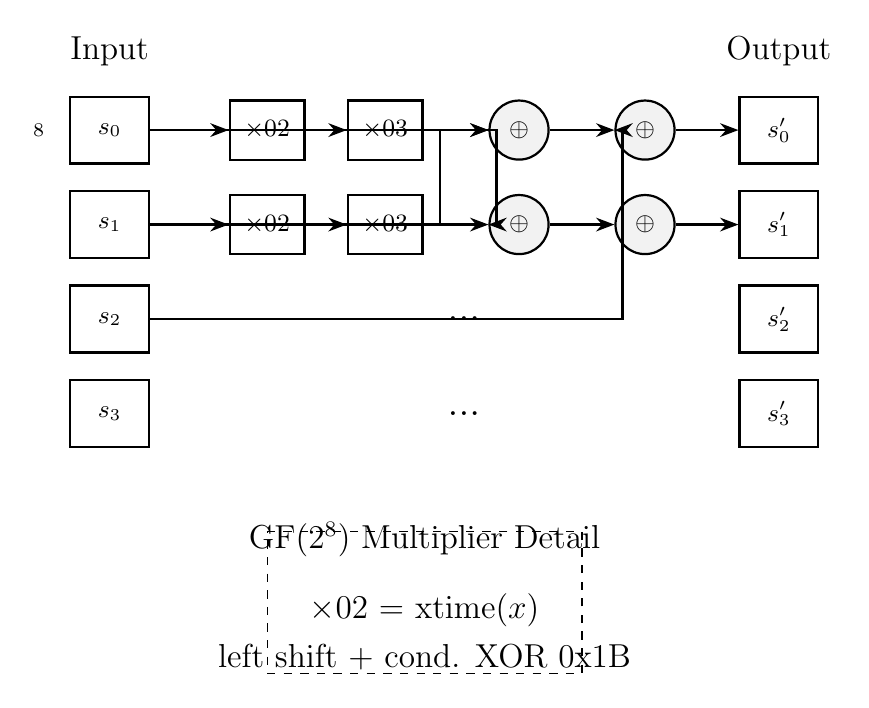
\begin{tikzpicture}

% Input bytes
\node[register] (s0) at (0,0) {$s_0$};
\node[register] (s1) at (0,-1.2) {$s_1$};
\node[register] (s2) at (0,-2.4) {$s_2$};
\node[register] (s3) at (0,-3.6) {$s_3$};

\node[font=\large, above=0.25cm of s0] {Input};
\node[buswidth] at (-0.9,0) {8};

% GF multipliers (first two rows)
\node[alu] (m02_0) at (2,0) {$\times$02};
\node[alu] (m03_0) at (3.5,0) {$\times$03};

\node[alu] (m02_1) at (2,-1.2) {$\times$02};
\node[alu] (m03_1) at (3.5,-1.2) {$\times$03};

\draw[wire] (s0) -- (m02_0);
\draw[wire] (s0.east) -- ++(0.6,0) |- (m03_0);
\draw[wire] (s1) -- (m02_1);
\draw[wire] (s1.east) -- ++(0.6,0) |- (m03_1);

% XOR trees (first two outputs)
\node[logic, circle, minimum size=0.75cm] (x0a) at (5.2,0) {$\oplus$};
\node[logic, circle, minimum size=0.75cm] (x0b) at (6.8,0) {$\oplus$};

\node[logic, circle, minimum size=0.75cm] (x1a) at (5.2,-1.2) {$\oplus$};
\node[logic, circle, minimum size=0.75cm] (x1b) at (6.8,-1.2) {$\oplus$};

\draw[wire] (m02_0) -- (x0a);
\draw[wire] (m03_1) -- ++(0.7,0) |- (x0a);
\draw[wire] (x0a) -- (x0b);
\draw[wire] (s2.east) -- ++(6,0) |- (x0b);

\draw[wire] (m02_1) -- (x1a);
\draw[wire] (s0.east) -- ++(4.4,0) |- (x1a);
\draw[wire] (x1a) -- (x1b);

% Output bytes
\node[register] (o0) at (8.5,0) {$s_0'$};
\node[register] (o1) at (8.5,-1.2) {$s_1'$};
\node[register] (o2) at (8.5,-2.4) {$s_2'$};
\node[register] (o3) at (8.5,-3.6) {$s_3'$};

\draw[wire] (x0b) -- (o0);
\draw[wire] (x1b) -- (o1);

\node[font=\Large] at (4.5,-2.4) {...};
\node[font=\Large] at (4.5,-3.6) {...};

\node[font=\large, above=0.25cm of o0] {Output};

% GF multiplier detail box
\node[draw, dashed, minimum width=4cm, minimum height=1.8cm] (detail) at (4,-6) {};
\node[font=\large, text centered] at (4,-5.2) {GF($2^8$) Multiplier Detail};
\node[font=\large, text centered] at (4,-6.1) {$\times$02 = xtime($x$)};
\node[font=\large, text centered] at (4,-6.7) {left shift + cond. XOR 0x1B};

\end{tikzpicture}
\end{document}
